\section{Justificativa} 
\label{justificativa}

A indústria de jogos digitais tem apresentado um crescimento contínuo, ganhando popularidade a cada ano e trazendo consigo novas oportunidades de negócio. Projeções da renomada empresa \textit{\gls{Newzoo}} indicam que o mercado de jogos \textit{mobile} poderá gerar uma receita aproximada de US\$ 103,1 bilhões até 2025 \cite{game_market_2022}. Este progresso não apenas reflete a crescente demanda por jogos \textit{mobile}, mas também revela a promissora lucratividade dentro deste segmento da indústria de jogos eletrônicos. A crescente popularidade dos jogos para dispositivos móveis, consoles de videogame e plataformas de PC evidencia esse crescimento. Em particular, o mercado de jogos para dispositivos móveis testemunhou um aumento significativo em 2020, impulsionado pelo aumento exponencial do número de usuários de \textit{smartphones} em todo o mundo. Além disso, o cenário dos jogos eletrônicos foi transformado pela ascensão das plataformas de \textit{streaming} de jogos, como o \textit{Google Stadia} e o \textit{Microsoft xCloud}, que permitem aos jogadores transmitir jogos diretamente pela internet, eliminando a necessidade de hardware de jogo de alta potência.

Paralelamente a esses avanços, os \textit{eSports}, também conhecidos como esportes eletrônicos, emergiram como uma forma popular e altamente lucrativa de entretenimento. Grandes torneios de \textit{eSports} atraem audiências globais significativas, proporcionando entretenimento cativante para os espectadores, ao mesmo tempo que oferecem prêmios em dinheiro substanciais para os jogadores profissionais. O futuro promissor dos \textit{eSports} parece ser delineado por uma trajetória ascendente, continuando a cativar públicos globais e inspirar investimentos inovadores em um ciclo virtuoso de crescimento econômico e excelência competitiva.

Nesse cenário, a plataforma \textit{\gls{Steam}}, um espaço virtual de destaque para distribuição de jogos para computadores, emerge como um reflexo do panorama mais amplo da indústria. Dados da \textit{\gls{SteamDB}} revelam um crescimento constante no lançamento de novos jogos na plataforma \textit{\gls{Steam}}. Somente em 2022, mais de 13 mil novos títulos foram introduzidos, indicando um progresso robusto nesse segmento específico em comparação com os anos anteriores. Essa expansão contínua, visualizada na Figura \ref{GameReleaseYear}, confirma a tendência de crescimento no mercado de jogos digitais.

\begin{figure}[H]
	\centering
	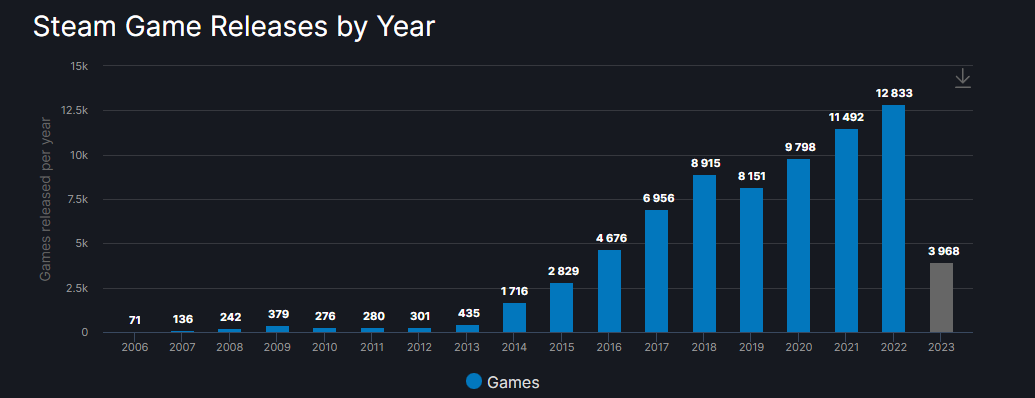
\includegraphics[scale=0.55]{./imagens/introducao/games_release_by_year.png}
	\caption{Steam Game Release Summary}
	\label{GameReleaseYear}
	\fonte{\cite{games_release_year}}
\end{figure}

Esse crescimento contínuo no mercado de jogos digitais é impulsionado pelo avanço tecnológico e pelo acesso generalizado à internet. A rápida penetração da internet na sociedade, como evidenciado por um estudo do \textit{\gls{DataReportal}}, mostra que aproximadamente 62,5\% da população mundial são usuários da internet, representando um aumento de 4\% em relação ao ano anterior \cite{digital_2022_global_overview_report}. No Brasil, o uso da internet está em constante ascensão, com pessoas entre 16 e 64 anos dedicando, em média, cerca de 10 horas diárias a atividades online \cite{digital_2022_global_overview_report}. O país se destaca como o terceiro no ranking mundial de tempo online, ficando atrás apenas da África do Sul e Filipinas, conforme evidenciado na Figura \ref{DailyTime}.

\begin{figure}[H]
	\centering
	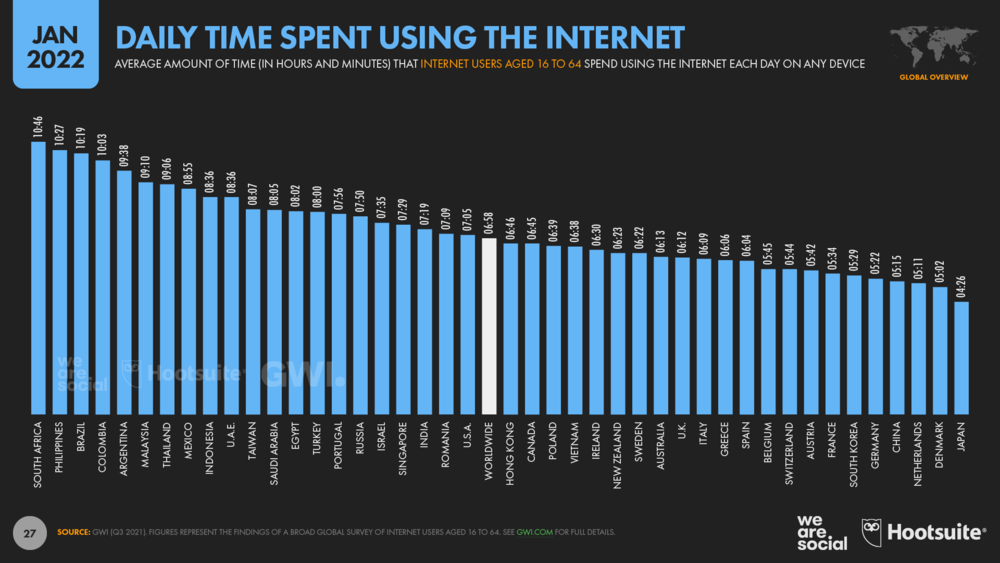
\includegraphics[scale=0.4]{imagens/introducao/daily_time_internet.png}
	\caption{Daily Time Spent Using The Internet}
	\label{DailyTime}
	\fonte{\cite{digital_2022_global_overview_report}}
\end{figure}

Esses dados indicam o Brasil como um mercado de grande potencial para produtos e conteúdos relacionados à internet, oferecendo um ambiente altamente favorável para iniciativas empreendedoras inovadoras. A mudança nos padrões de consumo, onde a conveniência e a acessibilidade proporcionadas pelas plataformas online desempenham um papel central, é particularmente evidente no cenário de jogos digitais. Este mercado em expansão, estimado em US\$ 323,5 bilhões até 2026 \cite{pesquisa_global_games}, requer soluções centralizadas para facilitar a gestão dos jogos para os entusiastas. Nesse contexto, a \textit{GameLocker} surge como uma solução ideal, não apenas para organizar os jogos, mas também para proporcionar um ambiente propício à interação entre jogadores, aproveitando ao máximo as oportunidades oferecidas por este mercado em expansão, as tendências atuais e se preparando para as futuras evoluções que certamente moldarão o futuro dos jogos eletrônicos.